\documentclass{article}

\usepackage{amsmath}
\usepackage{bm}
\usepackage{etoolbox}
\usepackage{hyperref}
\usepackage{listings}
\usepackage{multicol}
\usepackage{multido}
\usepackage{relsize}
\usepackage{tikz}
\usetikzlibrary{hobby}

\usepackage[utf8]{inputenc}
\usepackage[english]{babel}

\setlength{\parindent}{4em}
\setlength{\parskip}{1em}

\let\oldhat\hat
\renewcommand{\vec}[1]{\pmb{#1}}
\renewcommand{\hat}[1]{\oldhat{\pmb{#1}}}
\newcommand{\undersetvecexp}[4]{
  \underset{ \mathsmaller{#2 \times #3} }
           { \hphantom{{}^{#4}} \vec{#1} ^ {#4} }
}
\newcommand{\kunderset}[3]{
  \underset{ \mathsmaller{#2 \times #3} }
           { #1 }
}
\newcommand{\undersetvec}[3]{ \undersetvecexp{#1}{#2}{#3}{} }
\newcommand{\abs}[1]{\lvert #1 \rvert}
\newcommand{\lnorm}[2]{ {\left\lVert #2 \right\rVert}_#1 }
\newcommand{\lnormexp}[3]{ {\left\lVert #3 \right\rVert}_#1^#2 }
\newcommand{\bigbraces}[1]{ \left\{ #1 \right\} }
\newcommand{\bigbrackets}[1]{ \left[ #1 \right] }
\newcommand{\bigparens}[1]{ \left( #1 \right) }
\newcommand{\kpartial}[2]{ \frac{\partial \, #1}{\partial \, #2} }

\newcommand{\gausswithpeak}[4]{
  ( (#4) *
    (exp( ( -(#1-#2)^2 ) /
          ( 2*(#3^2)   )  ) ) )
}

\newcommand{\KLogisticPdf}[3]{
  % KLogisticPdf{mu}{sdev}{peak}
  (#3) * 4
  * exp( -(x-(#1)) /
          ((#2)*sqrt(3)/pi))
  / ((1 + exp(-(x-(#1)) /
               ((#2)*sqrt(3)/pi)) )**2)
}

\newcommand{\KLogisticCdf}[3]{
  % KLogisticCdf{mu}{sdev}{peak}
  (#3) /
  ( 1 + exp(-(x-(#1)) /
             ((#2)*sqrt(3)/pi)) )
}


\usepackage{graphicx}
\graphicspath{ {../plot_expers/images/} }

\usepackage{mathtools}

\title{CAAM 471/571: Traveling Salesman Project}
\date{2017-04-19}
\author{Kevin Burleigh and Julio Ledesma}

\begin{document}

\maketitle

\lstset{frame=tb,
  language=Python,
  aboveskip=5mm,
  belowskip=5mm,
  showstringspaces=false,
  columns=flexible,
  basicstyle={\small\ttfamily},
  numbers=none,
  numberstyle=\tiny\color{gray},
  keywordstyle=\color{blue},
  commentstyle=\color{lightgray},
  stringstyle=\color{brown},
  breaklines=true,
  breakatwhitespace=true,
  tabsize=3
}

\section{Problem Description}
\begin{flushleft}

We were tasked
to solve the Traveling Salesman Problem
using the branch-and-cut method,
utilizing Gurobi
to solve only linear programming relaxations of integer programs.

Given a graph $G = (N,E)$ with nodes $N$ and edges $E$,
and an associated cost $c_e$ for each edge,
the goal of the TSP
is to find the least costly path
which visits each node exactly once
and returns to the starting node
(a Hamiltonian cycle).

The TSP can be formulated
as the following integer program:
\begin{equation} \label{eq:tspip}
\begin{alignedat}{3}
 & \text{minimize}         & \sum_{e \in E}{c_e x_e} & \\
 & \text{subject to} \quad & \sum_{e \in \delta(\{n\})}{x_e} = 2, \quad & \forall n \in N \\
 &                   \quad & \sum_{e \in \delta(S)}{x_e} \geq 2,  \quad & \forall S \subset N, S \neq \emptyset \\
 &                         & x_e \in \{ 0,1 \}, \quad                     & \forall e \in E
\end{alignedat}
\end{equation}
where $x_e$ is a decision variable
indicating whether or not
the associated edge is part of the tour,
and $\delta(S)$ is the set of edges
in the cut of node set $S$.
The first set of constraints in \eqref{eq:tspip}
ensures that each node
is entered exactly once
and then exited exactly once.
This leaves open the possibilty of subtours,
which are eliminated by the second set of constraints.

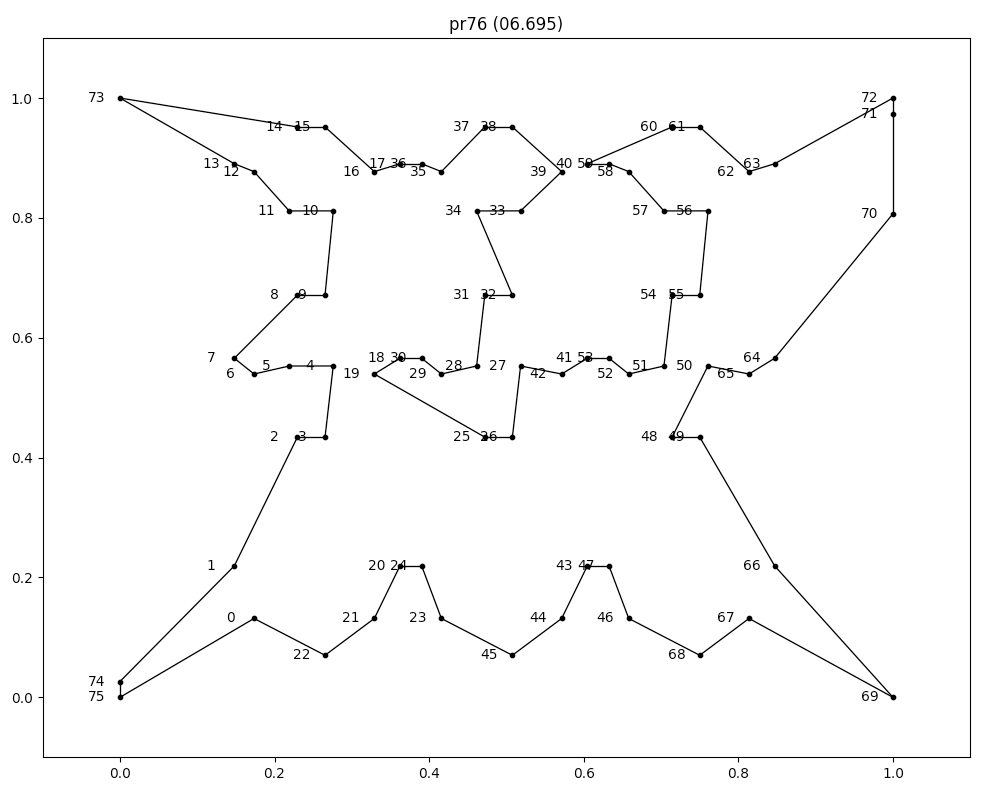
\includegraphics[width=4in, height=4in]{pr76_optTour}

\end{flushleft}

\section{Algorithm}

The algorithmic approach to solving TSPBC is as follows:
1. Initialize a Gurobi model with input data and add to a priority queue.
2. While the priority queue is not empty, pop a model off and set as current model
3. Process the current model i.e. adding constraints, and create new branches
4. For each new branch, add to priority queue
Each step in the algorithm will be explored in further detail.

\subsection{Main Loop}
\begin{flushleft}

The main control loop:

\begin{enumerate}
\item creates an initial model
\item adds the initial model to the model pool
\item until the model pool is empty:
  \begin{enumerate}
  \item removes a model from the pool
  \item processes the model
  \item adds any resulting new models (and their associated objective lower bounds) to the pool
  \end{enumerate}
\end{enumerate}

Processing ends when the model pool is empty.

\begin{lstlisting}
## tsp_solver.py
class TspBranchAndCut(object):
    def solve(self):
        initial_model = self.create_initial_model()
        self.add_model_to_pool(model=initial_model, obj_lb=-float('inf'))

        while not self.model_pool_is_empty():
            model = self.remove_next_model_from_pool()

            for obj_lb,new_model in self.process_model(model):
                self.add_model_to_pool(model=new_model, obj_lb=obj_lb)
\end{lstlisting}

\end{flushleft}


\subsection{The Initial Model}
\begin{flushleft}

The initial LP relaxation of \eqref{eq:tspip} is:
\begin{equation} \label{eq:tsplpinit}
\begin{alignedat}{3}
 & \text{minimize}         & \sum_{e \in E}{c_e x_e} & \\
 & \text{subject to} \quad & \sum_{e \in \delta(\{n\})}{x_e} = 2, \quad & \forall n \in N \\
 &                         & 0 \leq x_e \leq 1, \quad                     & \forall e \in E
\end{alignedat}
\end{equation}
where the decision variables $x_e$
are now allowed to take any value
between zero and one,
and the subtour constraints
have been removed
(they will gradually be re-introduced
as the algorithm progresses).

\begin{lstlisting}
## tsp_solver.py
class TspBranchAndCut(object):
    def create_initial_model(self):
        model = grb.Model('tsp')
        xx = model.addVars(self.edges,
            lb    = 0.0,
            ub    = 1.0,
            vtype = grb.GRB.CONTINUOUS,
            name  = 'xx',
            obj   = self.cost_by_edge
        )
        degree_constrs = model.addConstrs(
          (xx.sum(node,'*') + xx.sum('*',node) == 2.0 for node in self.nodes),
          'degree'
        )
        model.update()
        return model
\end{lstlisting}

\end{flushleft}

\subsection{Model Processing}
\begin{flushleft}

Once a model has been pulled
from the model pool,
it is optimized using gurobi.

If the model is infeasible,
or if it cannot possibly yield a new best tour
because its LP relaxation lower bound
is greater than the current best tour cost,
it is discarded
(the 'bound' part of branch-and-cut)
and processing stops.

If the current solution
is a valid tour
(and therefore integral)
with a cost less than that
of the current best tour,
the current solution becomes the new best tour
and processing stops.

Otherwise the current solution
either non-integral or not a tour,
so, if possible, new constraints
are added to the model
(the 'cut' part of branch-and-cut)
and it is re-optimized.
If no cuts could be added,
new variable fixing models
(where some non-integral $x_e$
is forced to take on a value of 0 or 1)
are created
and returned to the caller
(the 'branch' part of branch-and-cut).

\begin{lstlisting}
## tsp_solver.py
class TspBranchAndCut(object):
    def process_model(self, model):
        new_model_info = []
        while True:
            model.update()
            model.optimize()

            if self.solution_is_infeasible(model):
                break

            if not self.solution_can_become_new_best(model):
                break

            if self.solution_is_tour(model):
                if self.solution_is_new_best(model):
                    self.update_best(model)
                break

            if self.add_cuts_to_model(model):
                continue

            branch_models = self.create_branch_models(model)
            for branch_model in branch_models:
                new_model_info.append( (model.getAttr('ObjVal'), branch_model) )

            break

        return new_model_info
\end{lstlisting}
\end{flushleft}


Once we developed our algorithm for solving TSPBC,
we looked to Python and the gurobipy module.
Additionally, we implemented a Graph object
to facilitate our computation of TSPBC.
Graph is initialized
by helper functions
that assign its node, edge and edge weight attributes.
Graph also contains
methods to find the minimum cut,
to compute connected components,
and to determine if the instance forms a tour.
Instances of graph are copied
before more branches are produced.
Additionally, there are auxiliary functions
that easily convert
a Graph instance into a Gurobi model.

\section{Initialize model}
Given an input fie,
the data is translated
as a series of nodes,
edge and their assigned weights,
with each node having an edge
to every other node.
This data is transformed
into a Gurobi model,
initialized with degree constraints
and bounds on the edge decision variables.
This creates our initial linear program (LP)
for the TSPBC.
Our initial LP is then added to our priority queue.

\section{Process}
While the priority queue is not empty,
we pop a model
and set as our current model.
We then update the model
and solve for the optimal solution.
Before we start to branch,
we first check to see
whether the solution is feasible.
If infeasible,
we stop the branch
and move on to the next item in the priority queue.
Next, we check if the model
can be cut down
by adding constraints
that lower the objective function.
We then check
if our solution forms a tour,
else we stop the branch.
If possible,
we add new constraints
that help our model
reduce its objective value.
Once global and local constraints
are added to the models,
we create two new branches
and continue once again
for the next model
in the priority queue.

\section{Constraints}
These specific cuts
are comb and blossom inequalities,
integral and non-integral sub-tour constraints,
and mixed-integer Gomory cuts.
For the comb and blossom inequalities,
we searched for cuts based of this equation
in our candidate solution:
[INSERT BLOSSOM INEQUALITY]
For both integral and non-integral sub-tour constraints,
we check to see
if the current model formed a sub-tour,
and if so we added a constraint.
Lastly, for mixed integer Gomory cuts,
we searched for cuts based of
[INSERT MIXED INTEGER GOMORY CUTS].
For each cut,
constraints are added
to each Gurobi model
and the model is then solved
and branched out again.

\section{Min Cut}
To compute the min cut,
we use the Stoer-Wagner min-cut algorithm
in the provided paper.
Our implementation of this algorithm
returned the nodes that made up the min cut
as well as the size of the min cut.
The value of the minimum cut
was less than two
if and only if
there is a constraint that has been violated.
This function is contained as a method in Graph.

\section{Computing Tour}
Given a candidate branch,
we must check if it forms a potential solution.
In our python implementation,
our solution is a vector of values in [0.0, 1.0].
These values represent
if an edge is included in our solution.
We can eliminate infeasible branches
if their vector contains a value
that isn’t either 0.0 or 1.0.
Additionally, we need to check
if our potential solution satisfies
the degree constraint [degree].
Finally, we must check
that our candidate solution produces
at most one connected component.
We can compute the connected components
of our candidate solution
by running breadth-first search
on every edge in our candidate solution.
If our candidate solution passes
that each edge is either 0.0 or 1.0,
then we have each node in our tour
meeting the degree constraint [degree],
and that our candidate solution
forms at most one connected components [degree],
then this is sufficient to declare
our candidate solution a tour.
This function is contained as a method in Graph.

\section{Implementation}

\subsection{The Graph Class}

A \textit{Graph} class was created
to encapsulate purely graph-related functionality,
such as identifying:
\begin{enumerate}
\item nodes in connected components
\item edges in a min-cut
\item edges in the cut for a set of nodes
\item whether or not a set of edges forms a tour
\end{enumerate}

\section{Results}
    att48

    berlin52

    gr21

    hk48

    ulysses22

    pr76

    st70

\section{Improvements}

\section{Closing Remarks}
Our implementation of TSPBC was successful
in that we could correctly solve
each of the data sets provided.
However, as stated in our improvements section,
we could have added more types of cuts
to reduce the runtime of pr76.


\section{Section Title Here}

\subsection{Subsection Title Here}

\begin{flushleft}

Some text here.

\begin{equation} \label{probdef}
  p(a \le Z \le b) = \int_{a}^{\,b} \phi(x) \,dx
\end{equation}

Reference equation \autoref{probdef} here.

\begin{align*}
  p(a \le Z \le b)  &=  p(Z \le b) - p(Z \le a) \\
                    &=  \int_{-\infty}^{\,b} \phi(x) \,dx
                        -
                        \int_{-\infty}^{\,a} \phi(x) \,dx \\
                    &=  \Phi(b) - \Phi(a)
\end{align*}

Inline $\Phi(\alpha)$ here.

\begin{equation*}
  \Phi(\alpha)  = \int_{-\infty}^{\,\alpha} \phi(x) \,dx
\end{equation*}

% \begin{figure}[h!]
% \begin{center}
% \input{fig_pdfcdfarea}
% \caption{
% Image caption here.}
% \label{pdfcdfarea}
% \end{center}
% \end{figure}

\end{flushleft}

\end{document}
